\documentclass[a4paper,12pt]{article}
\usepackage[left=2cm,right=2cm,top=2cm,bottom=2cm]{geometry}
\usepackage{tikz}


\title{TikZ commends tutorial}
\date{\today}
\author{Yi-Chen Zhang}

\begin{document}
\maketitle
The TikZ commands can be inside the environment \textbackslash begin\{tikzpicture\} \ldots \textbackslash end\{tikzpicture\} or simply use \textbackslash tikz clause. We run \textsf{pdflatex} or \textsf{latex} followed by \textsf{dvips} to execute the TikZ commends. 

\section{Preliminary}
\subsection{Straight Path Construction}
%Let's get started with drawing a path. A path is a series of straight lines and curves that are connected. We start a path by specifying the coordinates of the start position as a point in brackets, as in $(0,0)$. The starting point is followed by a series of path extension operators `\textsf{-}\textsf{-}'. Then it must be followed by another coordinate and extends the path in a straight line to a new position. We can put some options in square brackets to describe the properties of the lines. This will be discussed later.
\begin{verbatim}
Useage:
  \draw[options] (x1,y1) -- (x2,y2) -- (x3,y3);

Example:
  \draw (-1.5,0) -- (1.5,0) -- (0,-1.5) -- (0,1.5);
  \draw[thick, rounded corners=10pt] 
    (0,0) -- (0,2) -- (1,3.25) -- (2,2) -- (2,0) -- (0,2) -- (2,2) -- (0,0) -- (2,0);
\end{verbatim}

\tikz \draw (-1.5,0) -- (1.5,0) -- (0,-1.5) -- (0,1.5);
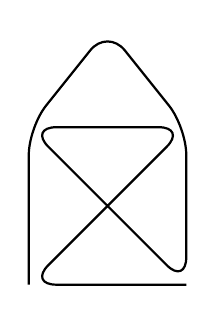
\begin{tikzpicture}
  \draw[thick, rounded corners=10pt] (0,0) -- (0,2) -- (1,3.25) -- (2,2) -- (2,0) -- (0,2) -- (2,2) -- (0,0) -- (2,0); % -- cycle;
\end{tikzpicture}

\subsection{Circle Path Construction}
\begin{verbatim}
Usage:
  \draw[options] (x,y) circle (raidus);
  \draw[options] (x,y) ellipse (raidus1 and radius2);

Example:
  \draw (0,0) circle (2pt);
  \draw[red] (1,0) circle (3pt);
  \draw[fill=red] (2,0) circle (4pt);
  \draw[red,fill=red] (3,0) circle (5pt);
  \filldraw[blue,rotate=30] (3.5,-2) ellipse (10pt and 5pt);
\end{verbatim}


\begin{tikzpicture}
  \draw (0,0) circle (2pt);
  \draw[red] (1,0) circle (3pt);
  \draw[fill=red] (2,0) circle (4pt);
  \draw[red,fill=red] (3,0) circle (5pt);
  \filldraw[blue,rotate=30] (3.5,-2) ellipse (10pt and 5pt);
\end{tikzpicture}

\subsection{Curved Path Construction}
\begin{verbatim}
Usage:
  \draw[options] (x1,y1) .. controls (x2,y2) and (x3,y3) .. (x4,y4)

Example:
  \filldraw[gray] (0,0) circle (2pt) (1,1) circle (2pt)
                  (2,1) circle (2pt) (2,0) circle (2pt);
  \draw (0,0) .. controls (1,1) and (2,1) .. (2,0);
\end{verbatim}

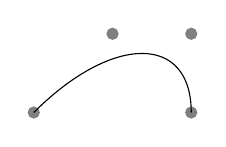
\begin{tikzpicture}
  \filldraw[gray] (0,0) circle (2pt)
                  (1,1) circle (2pt)
                  (2,1) circle (2pt)
                  (2,0) circle (2pt);
  \draw (0,0) .. controls (1,1) and (2,1) .. (2,0);
\end{tikzpicture}

\subsection{Rectangle Path Construction}
\begin{verbatim}
Usage:
  \draw[options] (x1,y1) rectangle (x2,y2);

Example:
  \draw (-1.5,0) -- (1.5,0);
  \draw (0,-1.5) -- (0,1.5);
  \draw[rotate=30, fill=red] (-0.5,-0.5) rectangle (-1,-1);
\end{verbatim}

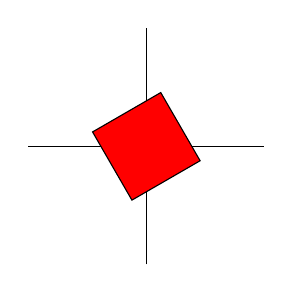
\begin{tikzpicture}
  \draw (-1.5,0) -- (1.5,0);
  \draw (0,-1.5) -- (0,1.5);
  \draw[rotate=30, fill=red] (-0.5,-0.5) rectangle (0.5,0.5);
\end{tikzpicture}

\subsection{Grid Path Construction}
\begin{verbatim}
Usage:
  \draw[options] (x1,y1) grid (x2,y2); 
\end{verbatim}

\begin{verbatim}
Example:
  \draw[step=.5cm, gray, very thin] (-1.4,-1.4) grid (1.4,1.4);
  \draw (-1.5,0) -- (1.5,0);
  \draw (0,-1.5) -- (0,1.5);
  \draw (0,0) circle (1cm);
  \draw[step=2pt] (0,0) grid (10pt,10pt);
\end{verbatim}

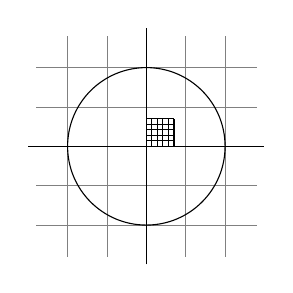
\begin{tikzpicture}
	\draw[step=.5cm, gray, very thin] (-1.4,-1.4) grid (1.4,1.4);
	\draw (-1.5,0) -- (1.5,0);
	\draw (0,-1.5) -- (0,1.5);
	\draw (0,0) circle (1cm);
  \draw[step=2pt] (0,0) grid (10pt,10pt);
\end{tikzpicture}

\subsection{Adding a Touch Style}
\noindent 
\textsf{Styles} are predefined sets of options that can be used to organize how a graphic is drawn. To define a style globally, we can use the \textbackslash tikzset command at the beginning of the document.
\begin{verbatim}
Usage:
  \tikzset{style_name./style={options}}

Example:
  \tikzset{blue_thin_lines/.style={color=blue!50,very thin}}
  \begin{tikzpicture}
    \draw[blue_thin_lines] (0,0) grid (5,5);
  \end{tikzpicture}
\end{verbatim}

\tikzset{blue_thin_lines/.style={color=blue!50,very thin}}
\begin{tikzpicture}
	\draw[step=0.5cm, blue_thin_lines] (0,0) grid (2,2);
\end{tikzpicture}\\

\noindent To define a style locally, we use a pair of square bracket ``[ ]'' to define styles at the beginning of a picture.
\begin{verbatim}
Usage:
  [style_name/.style={options}]

Example:
  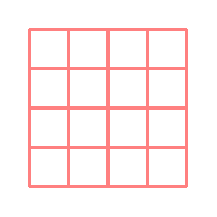
\begin{tikzpicture}
    [red_thick_lines/.style={color=red!50,very thick}]
    \draw[step=0.5cm, red_thick_lines] (0,0) grid (2,2);
  \end{tikzpicture}
\end{verbatim}

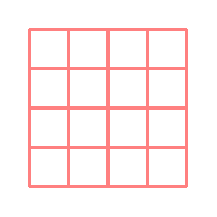
\begin{tikzpicture}
	[red_thick_lines/.style={color=red!50,very thick}]
	\draw[step=0.5cm, red_thick_lines] (0,0) grid (2,2);
\end{tikzpicture}\\

\noindent One can also define styles hierarchically.
\begin{verbatim}
Usage:
  \tikzset{style_name1/.style={style_name2, options}}

Example:
  \tikzset{green_help_lines/.style={help lines, color=green!90}}
  \begin{tikzpicture}
    \draw[step=0.5cm, green_help_lines] (0,0) grid (5,5);
  \end{tikzpicture}
\end{verbatim}

\tikzset{green_help_lines/.style={help lines, color=green!90}}
\begin{tikzpicture}
  \draw[step=0.5cm, green_help_lines] (0,0) grid (2,2);
\end{tikzpicture}\\

\clearpage
\newpage

\noindent Styles can also be used with a parameter.
\begin{verbatim}
Usage:
  [style_name/.style={options}, style_name/.default={options}]

Example:
  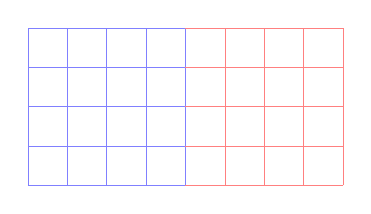
\begin{tikzpicture}
    [para_color/.style={help lines,color=#1!50}, para_color/.default=blue]
    \draw[step=0.5cm, para_color] (0,0) grid (2,2);
    \draw[step=0.5cm, para_color=red] (2,0) grid (4,2);
  \end{tikzpicture}
\end{verbatim}

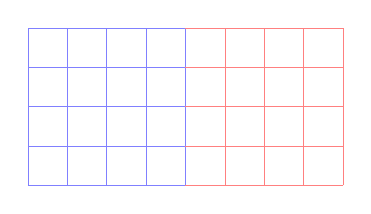
\begin{tikzpicture}
  [para_color/.style={help lines,color=#1!50}, para_color/.default=blue]
  \draw[step=0.5cm, para_color] (0,0) grid (2,2);
  \draw[step=0.5cm, para_color=red] (2,0) grid (4,2);
\end{tikzpicture}

\end{document}
